\documentclass[11pt, oneside]{book}
\usepackage{xcolor, indentfirst, setspace, graphicx, float}
\usepackage[margin=1.5in]{geometry}
\usepackage{titlesec}
\titleformat{\chapter}[display]
{\normalfont\bfseries\filcenter}
{\LARGE \thechapter}
{1ex}
{\titlerule[2pt]
\vspace{2ex}%
\LARGE}
[\vspace{1ex}%
{\titlerule[2pt]}]

\begin{document}

\newcommand*{\titleGP}{\begingroup % Create the command for including the title page in the document
		\centering % Center all text
		\vspace*{\baselineskip} % White space at the top of the page

		\rule{\textwidth}{1.6pt}\vspace*{-\baselineskip}\vspace*{2pt} % Thick horizontal line
		\rule{\textwidth}{0.4pt}\\[\baselineskip] % Thin horizontal line

		{\LARGE FRENCH COURSE NOTES}\\[0.2\baselineskip] % Title

\rule{\textwidth}{0.4pt}\vspace*{-\baselineskip}\vspace{3.2pt} % Thin horizontal line
\rule{\textwidth}{1.6pt}\\[1.5\baselineskip] % Thick horizontal line

\scshape % Small caps
FSF 2D7 AND FSF 3U7\\[0.7\baselineskip]
\today \par % Location and year

\vspace*{2\baselineskip} % Whitespace between location/year and editors

\vspace{0.7\baselineskip}
{\Large ANDREW WANG\par}
{\Large MAAS LALANI\par}
{\Large SCOTT MCNEIL\par} % Editor list

\vfill % Whitespace between editor names and publisher logo

\endgroup}
\titleGP


\tableofcontents

\setstretch{1.5}
\chapter{Verbs}
\section{L'infinitif}
The \textit{infinitive} tense is to describe an action where no one is performing the action. In English, the word to always precedes the verb in infinitive form. In French, verbs in the \textit{infinitive} virtually always have any one of the three following endings \textit{er, ir, re}. 
\vspace{\baselineskip}
For example:

\begin{enumerate}
    \item[Monter] - to climb
	\item[Falloir] - to have to
	\item[Boire] - to drink
	\item[Ha\"ir] - to hate
\end{enumerate}

The \textit{infinitive} is not conjugated| instead, it is used in the same form regardless of the pronouns used along with it. Tenses will be covered starting from the next part of this chapter, beginning with the present tense.

\section{Le pr\'esent de l'indicatif}

The present tense is one of the most commonly used tenses in French, due to its various uses. Consider the following cases:

\begin{description}
	\item[1. Current actions and situations] 

		\begin{itemize}
			\textcolor{white}{a} 
			\item[] E.g., \texttt{I am tired.} $\rightarrow$ \texttt{Je suis fatigu\'e.}
			\item[] \texttt{we go to the market.} $\rightarrow$ \texttt{nous allons au march\'e.}
		\end{itemize}
		
	\item[2. Habitual actions]
	
		\begin{itemize}
			\textcolor{white}{a} 
			\item[] E.g., \texttt{he goes to school every day.} $\rightarrow$ \texttt{il va \`a l'\'ecole chaque jour.}
			\item[] \texttt{we go to the market.} $\rightarrow$ \texttt{nous allons au march\'e.}
		\end{itemize}
	
	
	\item[3. Absolute and general truths]
	
		\begin{itemize}
			\textcolor{white}{a} 
			\item[] E.g., \texttt{the earth is spherical.} $\rightarrow$ \texttt{la terre est sph\'erique.}
			\item[] \texttt{education is important.} $\rightarrow$ \texttt{l'\'education est importante.}
		\end{itemize}
		
	\item[4. Actions which will occur immediately]
	
		\begin{itemize}
			\textcolor{white}{a} 
			\item[] E.g., \texttt{I'll be right there!} $\rightarrow$ \texttt{j'arrive!}
			\item[] \texttt{He is leaving right away} $\rightarrow$ \texttt{il part tout de suite}
		\end{itemize}
		
	\item[5. Conditions, such as in \textit{si} clauses]
	
		\begin{itemize}
			\textcolor{white}{a} 
			\item[] E.g., \texttt{if I can, I will go with you} $\rightarrow$ \texttt{si je peux, j'irai avec toi}
			\item[] \texttt{if you like.} $\rightarrow$ \texttt{si vous voulez.}
		\end{itemize} 
		
\end{description}

Note that the present tense is not used after certain constructions that indicate an action that will occur in the future, such as \textit{apr\`es que} (after) and \textit{aussit\^ot que} (as soon as).

As mentioned in section 1.1, verbs virtually always end in \textit{er, ir}, or \textit{re}. Each type of ending has its own conjugation rule.

\begin{enumerate}
	\item[\textbf{ER}] to conjugate a regular \textit{-er} verb, drop the \textit{-er} off of the \textit{infinitive} to get the stem or \textit{radical}. The add the appropriate ending that agrees with the subject: \textit{E}, \textit{ES}, \textit{E, ONS, EZ}, and \textit{ENT}
	
	For example, consider the verb \textit{aimer}:
	\begin{figure}[H]
	
\includegraphics[scale=0.8]{charts/ERpresent.png}
	\end{figure}
	
	\item[\textbf{IR}] to conjugate a regular \textit{-ir} verb, drop the \textit{-ir} and add the correct ending that agrees with the subject: \textit{IS, IS, IT, ISSONS, ISSEZ, ISSENT}

	For example, consider the verb \textit{choisir}:
	\begin{figure}[H]
	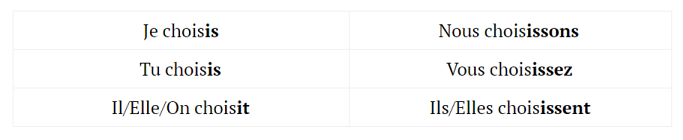
\includegraphics[scale=0.8]{charts/IRpresent.png}
	\end{figure}
	
	\item[\textbf{RE}] to conjugate a regular -re verb replace the -re with the appropriate ending:
S, S, -, ONS, EZ, ENT

	For example, consider the verb \textit{descendre}:
	\begin{figure}[H]
	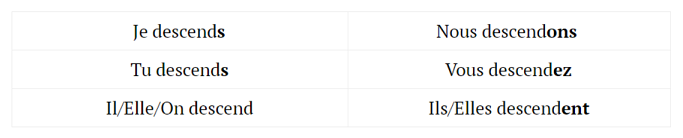
\includegraphics[scale=0.8]{charts/REpresent.png}
	\end{figure}
	
\end{enumerate}

\newpage

Irregular verbs in the present tense include: \textit{avoir, \^etre, faire, aller, savoir, pouvoir, dire} and \textit{vouloir}. 

	Here are their conjugations in the present tense: 
	
	\begin{figure}[H]
	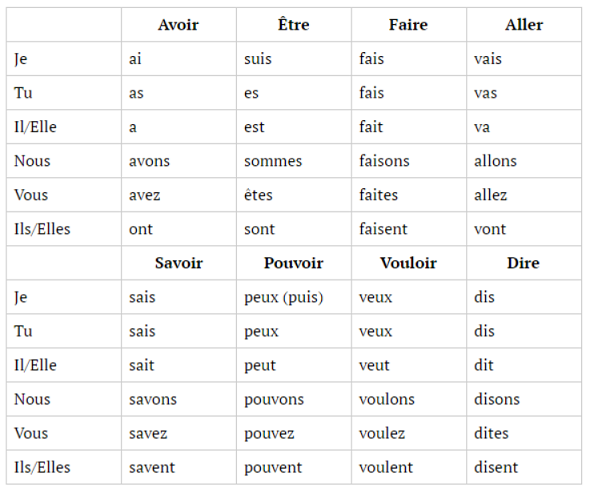
\includegraphics[scale=0.75]{charts/presentIrregular.png}
	\end{figure}
	{\let\thefootnote\relax\footnote{\textit{puis} is the form of \textit{pouvoir} used when making an inverse with \textit{je}. For example, \texttt{puis-je aller aux toilettes ?}}

\section{Le participe pass\'e}

The \textit{participe pass\'e} is a form of a verb combined with auxiliaries used in many compound tenses (tenses with an auxiliary, and therefore two conjugated elements, instead of one) such as the \textit{pass\'e compos\'e, condtionnel pass\'e, plus-que-parfait,} and \textit{futur ant\'erieur}(all explained later this chapter). 

If, say, we were conjugating \textit{aimer} into the \textit{pass\'e compos\'e} (see section 1.4), we would use the auxiliary, \textit{avoir}, in the present tense (see section 1.2), along with the \textit{participe pass\'e} of {aimer}. \vspace{0.5\baselineskip}

For verbs ending in ER, the \textit{participe pass\'e} is simply formed by removing the ER of the infinitive form and adding an \textit{\'e}. \vspace{0.5\baselineskip}

For example, the \textit{participe pass\'e} of \textit{aimer} is \textit{aimé}. \vspace{0.5\baselineskip}

For verbs ending in IR, the \textit{participe pass\'e} is simply formed by removing the IR of the infinitive form and adding an \textit{i}. \vspace{0.5\baselineskip}

For example, the \textit{participe pass\'e} of \textit{finir} is \textit{fini}.\vspace{0.5\baselineskip}

For verbs ending in RE, the \textit{participe passé} is simply formed by removing the RE of the infinitive form and adding a \textit{u}. \vspace{0.5\baselineskip}

For example, the \textit{participe pass\'e} of \textit{rendre} is \textit{rendu}.  \vspace{0.5\baselineskip}

However, there are quite a few verbs with irregular \textit{participe pass\'e} forms: \vspace{0.5\baselineskip}


	\begin{figure}[H]
	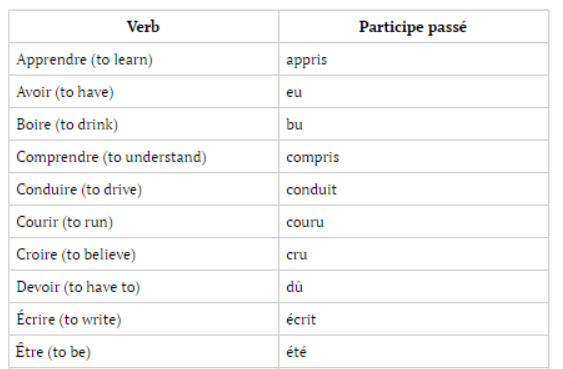
\includegraphics[scale=0.75]{charts/participePasseIrregular.png}
	\end{figure}
	
	\begin{figure}[H]
	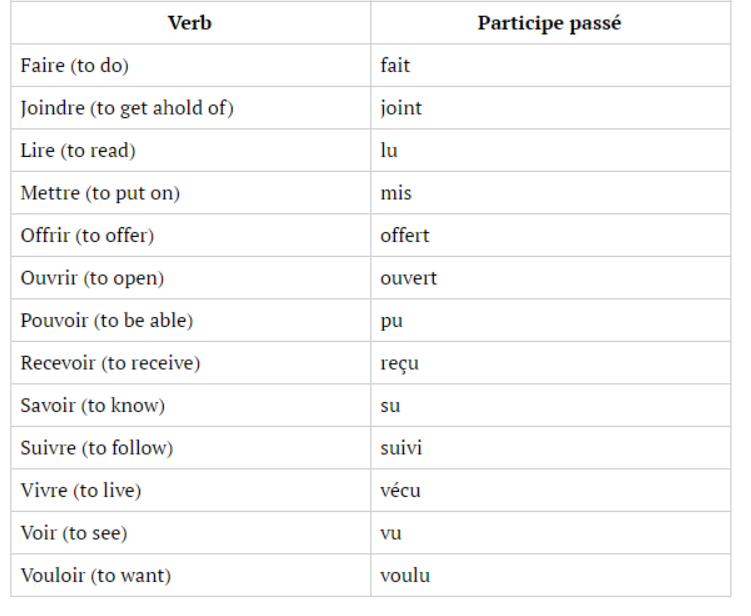
\includegraphics[scale=0.565]{charts/participePasseIrregular2.png}
	\end{figure}
	
\section{Le pass\'e compos\'e}

The \textit{pass\'e compos\'e} is used to describe something that happened and was completed in the past. In English, the equivalent form is a verb ending in \textit{-ed}. \vspace{0.5\baselineskip}

For example, \texttt{arrived, studied}. Note that many irregularities in English exist, e.g., saw and found. \vspace{0.5\baselineskip}

The \textit{pass\'e compos\'e} is conjugated using two parts: the \textit{auxiliaire} (auxiliary) and the \textit{participe pass\'e}. The auxiliary can be either the verb \textit{être} or \textit{avoir} conjugated in the present tense in accordance with the subject pronoun. The \textit{participe pass\'e} follows the auxiliary, which follows the subject pronoun. \vspace{0.5\baselineskip}

Say, we are trying to translate the sentence \texttt{"I studied three hours last night"} into French. We first note that the translation will be in a past tense since the verb \textit{to study} is in its past tense (pluperfect) form, \textit{studied}. The subject in question here is \textit{I}, which translates to \textit{je}. Also note that \textit{\'etudier}, the French word meaning \textit{to study} uses the auxiliary \textit{avoir}. \vspace{0.5\baselineskip}

\textcolor{red}{I} \textcolor{cyan}{studied} \textcolor{magenta}{for three hours} \textcolor{orange}{last night}  \vspace{0.5\baselineskip}

$\rightarrow$\textcolor{red}{J'} \textcolor{cyan}{ai \'etudi\'e} \textcolor{magenta}{pendant trois heures} \textcolor{orange}{hier soir} \vspace{0.5\baselineskip} 

The negative form of the sentence is formed through the placement of \textit{ne} and its partner, usually \textit{pas} around the auxiliary and potential pronouns. This is the case for negation of all compound cases and constructions involving two verbs. \vspace{0.5\baselineskip}

For instance, \texttt{Je \textcolor{red}{n}'ai \textcolor{red}{pas} \'etudi\'e pendant trois heures.}  \vspace{0.5\baselineskip}

Some verbs use \^etre as their auxiliary|. Here's a useful mnemonic to remember the most common of such verbs:
\textsc{DR. MRS. VANDERTRAMP}. These are generally \textit{intransitive} verbs — verbs that take an indirect object (See section . 3.1). What's even more tricky is that some verbs, such as \textit{descendre} can take both auxiliaries, depending on the context and the meaning of the verb in the context.

\begin{figure}[H]
	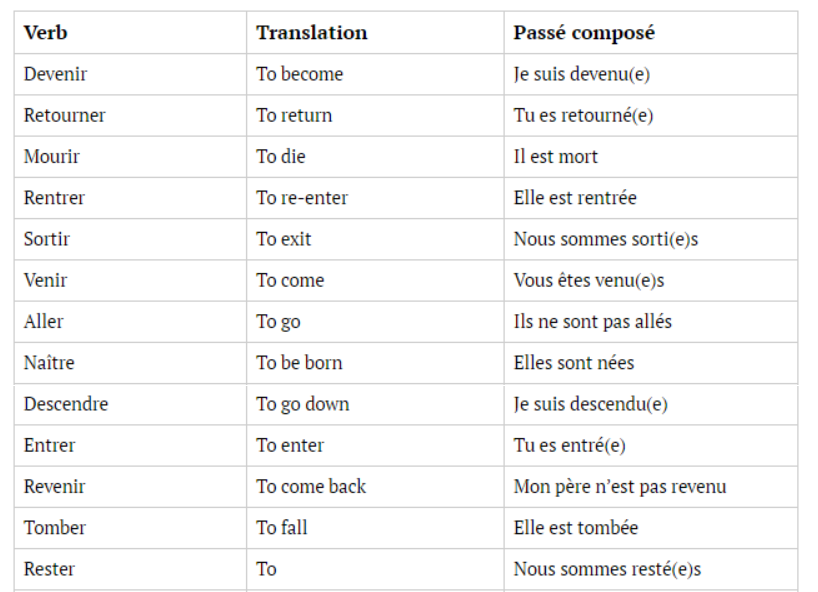
\includegraphics[scale=0.5]{charts/vandertramp.png}
\end{figure}
\begin{figure}[H]
	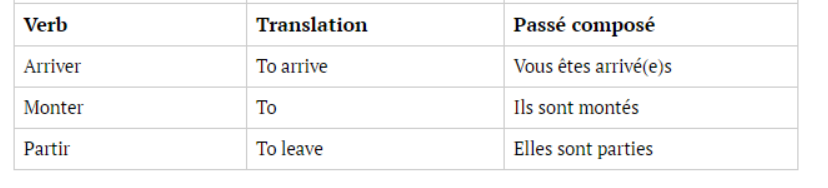
\includegraphics[scale=0.5]{charts/vandertramp2.png}
\end{figure}

Some verbs have irregular \textit{participe pass\'e}'s| refer to section 1.3
for details.

\section{Le futur simple}

The \textit{futur simple} is used to describe future events that will occur at a time that may not necessarily be in the near future (for events that will necessarily occur in the near future use the futur proche: aller (present tense) + infinitive, with no exceptions). The equivalent form in English is \textit{will} + \textit{main verb}. \vspace{0.5\baselineskip}

	For instance, \texttt{I will walk the dog}. \vspace{0.5\baselineskip}

	An important difference between the English future tense and the \textit{futur simple} lies in constructions beginning in \textit{apr\`es que} (after), \textit{aussit\^ot que} (as soon as), \textit{d\`es que} (as soon as), \textit{lorsque} (when), and \textit{quand} (when). An English speaker might say ``\texttt{as soon as he arrives, we eat.}" Note that \textit{to arrive} is conjugated in the present tense. A French speaker might say ``\texttt{quand il arrivera, nous mangerons}". Here, both verbs, \textit{arriver} and \textit{manger}, are conjugated in the \textit{futur simple}. \vspace{0.5\baselineskip}

With the exception of irregular verbs and verbs ending in RE, radicals of verbs in the \textit{futur simple} are the simply the infinitives of the verbs. \vspace{0.5\baselineskip}

For example, the radical of \textit{aimer} in \textit{futur simple} is \textit{aimer}. \vspace{0.5\baselineskip}

In the case of verbs ending in RE, simply removing the final \textit{e} gives us the desired radical. \vspace{0.5\baselineskip}

For example, the radical of \textit{perdre} in \textit{futur simple} is \textit{perdr}.  \vspace{0.5\baselineskip}

There is one set of endings for all verbs: \vspace{0.5\baselineskip}

\begin{figure}[H]
	
\includegraphics[scale=0.65]{charts/futurEndings.png}
\end{figure} \vspace{0.5\baselineskip}

In fact, these endings resemble the present tense (see section 1.2) conjugations of \textit{avoir} (with the exception of \textit{nous} and \textit{vous} which do not have the \textit{av-})! \vspace{0.5\baselineskip}

Adding together the radicals and endings forms the \textit{futur simple}.  \vspace{0.5\baselineskip}

For example, \texttt{my dad will give me some lunch money $\rightarrow$ mon p\`ere me donnerai un peu de l'argent pour le d\'ejeuner}. \vspace{0.5\baselineskip}

The irregular verbs have different radicals: \vspace{0.5\baselineskip}

\begin{figure}[H]
	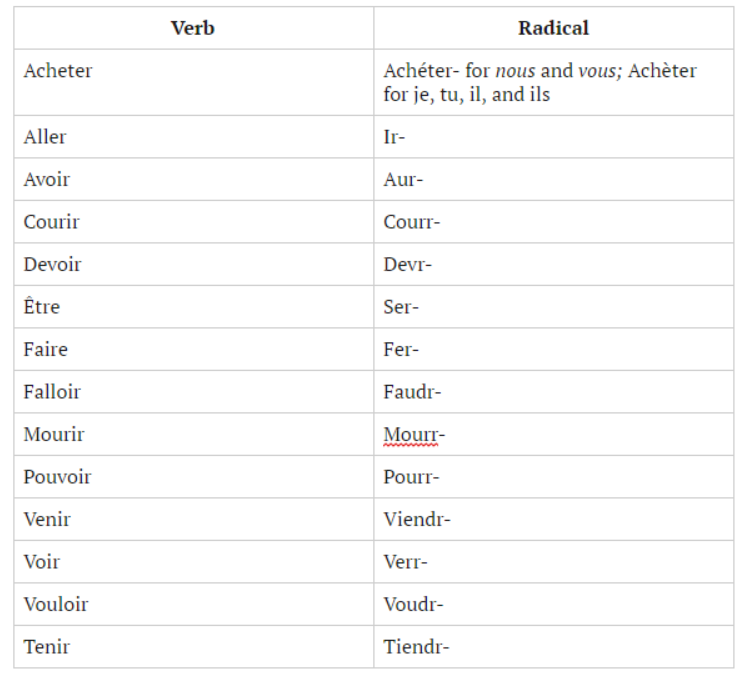
\includegraphics[scale=0.5]{charts/futurIrregular.png}
\end{figure} \vspace{0.5\baselineskip}


\section{L'imparfait}

The \textit{imperfect} tense (\textit{l'imparfait}) expresses a fact or an action that has already happened, similar to \textit{pass\'e compos\'e}, but can indicate an ongoing state of being or a repeated or incomplete action. Essentially, there isn't too much emphasis on whether the action has terminated. \vspace{0.5\baselineskip}

The imperfect tense can be used to indicate any of the following:

\begin{description}
	\item[1. Habitual actions or states of being] 

		\begin{itemize}
			\textcolor{white}{a} 
			\item[] E.g., \texttt{when I was young, we used to dance everyday} $\rightarrow$ \texttt{quand j'\'etais jeune, nous dansions chaque jour.}
		\end{itemize}
		
	\item[2. Physical and emotional descriptions including time, weather, \\ and feelings] 

		\begin{itemize}
			\textcolor{white}{a} 
			\item[] E.g., \texttt{When he was 3, he was always asleep} $\rightarrow$ \texttt{quand il avait 3 ans, il \'etait toujours endormi.}
		\end{itemize}
		
	\item[3. Actions or states of an unspecified duration] 
	
		\begin{itemize}
			\textcolor{white}{a} 
			\item[] E.g., \texttt{he was hoping to see you before you left.} $\rightarrow$ \texttt{il esp\'erait te voir avant que tu es parti.}
		\end{itemize}
		
	\item[4. Background information in conjunction with the \textit{pass\'e compos\'e}] 
	
		\begin{itemize}
			\textcolor{white}{a} 
			\item[] E.g., \texttt{I was at the park when he left.} $\rightarrow$ \texttt{j'\'etais au parc quand il est parti..}
		\end{itemize}
	
	\item[5. Wishes or suggestions] 
	
		\begin{itemize}
			\textcolor{white}{a} 
			\item[] E.g., \texttt{you could add more salt} $\rightarrow$ \texttt{tu pouvais mettre plus de sel}
		\end{itemize}
		
		
	\item[6. Conditions in \textit{si} clauses] 
	
		\begin{itemize}
			\textcolor{white}{a} 
			\item[] E.g., \texttt{if I were rich, I would visit Paris} $\rightarrow$ \texttt{si j'\'etais riche, je visiterais le Paris.}
		\end{itemize}
		
	\item[7. The expressions \textit{\^etre en train de} and \textit{venir de} in the past
] 
	
		\begin{itemize}
			\textcolor{white}{a} 
			\item[] E.g., \texttt{I was (in the process of) doing my homework.} $\rightarrow$ \texttt{j'\'etais en train de faire mes devoirs.}
		\end{itemize}
			
		
\end{description}

\section{Le conditionnel pr\'esent} 

The \textit{conditionnel pr\'esent} is used to describe a wish in a polite manner or a hypothetical situation that is usually not verifiable (an eventuality). In English, the equivalent form is a verb preceded by would, could, or even might. \vspace{0.5\baselineskip}

For example, the impact of an asteroid would push the two celestial bodies closer together. \vspace{0.5\baselineskip}

The radical of the \textit{conditionnel pr\'esent} tense is that of the \textit{futur simple} tense (see section 1.5). \vspace{0.5\baselineskip}

The endings of the \textit{conditional pr\'esent} tense are those of the \textit{l'imparfait} tense (see section 1.6).  \vspace{0.5\baselineskip}

Here are all the conjugations for \textit{avoir}, which has an irregular radical in the \textit{futur simple}, and therefore the \textit{condtionnel pr\'esent}:  \vspace{0.5\baselineskip}

\begin{figure}[H]
	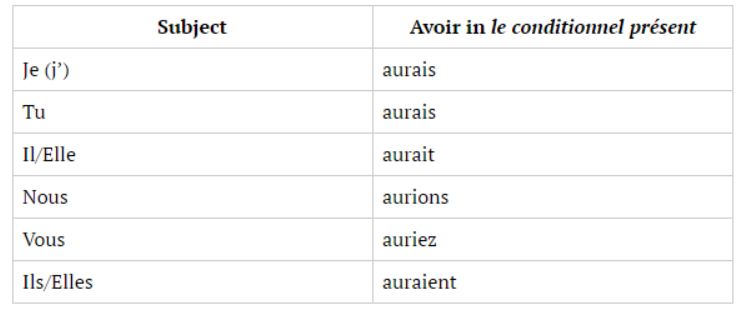
\includegraphics[scale=0.6]{charts/conditionnelAvoir.png}
\end{figure} \vspace{0.5\baselineskip}


The phrase ``\texttt{if \ldots then I would \ldots}”, is said to be incomplete without a clause from ``\textit{then I would \ldots} and on. \vspace{0.5\baselineskip}
 
For example, “\texttt{if I said I were free}” does not express a complete idea and is not a complete sentence. To complete the sentence, we would have to add a possibility, or an outcome of such a hypothetical situation. For instance, ``\texttt{if I said I were free, I would be a liar}". It may now be apparent that the “\textit{would be}” would be expressed in the \textit{conditionnel pr\'esent} tense, which it is. The translation is as follows: “\texttt{Si je disais que je suis libre, je serais un menteur.
}” Notice the use of \textit{condtionnel pr\'esent}, \textit{serais} (\^etre). \vspace{0.5\baselineskip}

In general, the construction is \textit{si + imparfait \ldots , conditionnel pr\'esent} \vspace{0.5\baselineskip}

For example, \texttt{if I had a million dollars, I would buy a yacht $\rightarrow$ si j'avais un million de dollars, j'ach\`eterai un yacht.} \vspace{0.5\baselineskip}

Note that a verb in the \textit{conditionnel pr\'esent} tense is never preceded by \textit{si}. 


\section{Le pr\'esent du subjonctif}

The \textit{subjonctif} expresses obligation and necessity (or, generally speaking, ideas that are subjective or uncertain). Certain expressions ending in \textit{que} must be followed by a verb in the \textit{pr\'esent du subjonctif} tense. \vspace{0.5\baselineskip} 

For example, \textit{il faut que, pour que, je veux que} etc.  \vspace{0.5\baselineskip}

The radical of a verb in the \textit{pr\'esent du subjonctif}  is given by removing the \textit{-ent} from the third person plural form (they, ils, elles) of the main verb in present tense.  \vspace{0.25\baselineskip}

For instance, the radical of \textit{aider} is formed by removing the \textit{-ent} from \textit{aident}, which is the third person plural form of \textit{aider} in the present tense. Therefore, the radical of \textit{aider} in the \textit{pr\'esent du subjonctif} is \textit{aid}.  \vspace{0.5\baselineskip}

The \textit{pr\'esent du subjonctif} has one set of endings for almost all verbs: \vspace{0.5\baselineskip}

\begin{figure}[H]
	
\includegraphics[scale=0.6]{charts/subjonctifEndings.png}
\end{figure} \vspace{0.5\baselineskip}

For example, \texttt{it is necessary that we leave $\rightarrow$ il faut que nous partions}.

The irregular verbs have different radicals: 
\begin{figure}[H]
	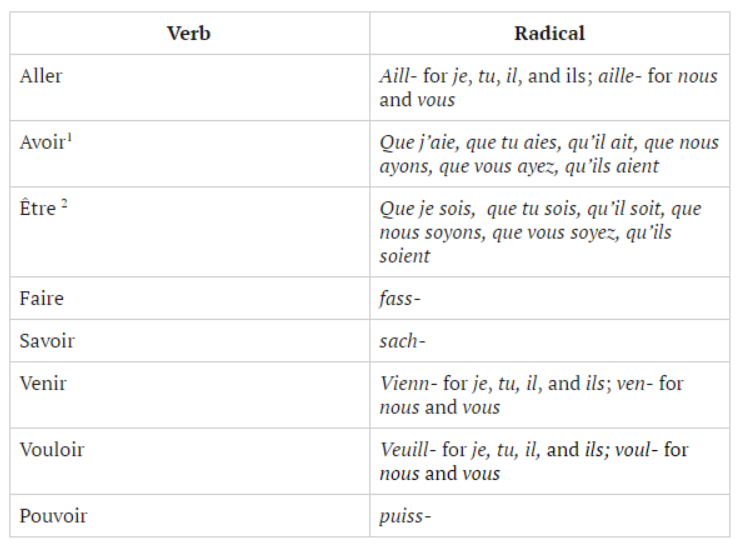
\includegraphics[scale=0.6]{charts/subjonctifIrregulars.png}
\end{figure} \vspace{0.5\baselineskip}

For example, \texttt{it is necessary that I be diligent so that I can ace my exams $\rightarrow$ il faut que je sois assidu pour que je puisse cartonner mes examens} 	

{\let\thefootnote\relax\footnote{avoir and \^etre are highly irregular in the subjunctive tense; conjugations given instead of radicals}

\section{Le participe pr\'esent}
The \textit{participe pr\'esent} is used to describe something that progresses. In English, the equivalent form is a verb ending in \textit{-ing}. For instance: doing, eating. Note that verbs in this form are usually preceded by the verb \textit{to be} e.g., I am doing, he is eating. \vspace{0.5\baselineskip}

The radical of the \textit{participe pr\'esent} derives from the first person plural form (we, nous) of the verb in the present tense of the verb in question. After the removing the -ons, we get the desired radical. \vspace{0.5\baselineskip}

Verbs in the \texttt{participe pr\'esent} form end in \textit{-ant}. \vspace{0.5\baselineskip}

Say we are trying to conjugate \textit{manger}. We word first consider the first person plural form (we, nous) of the verb in the present tense, \textit{mangeons}, and remove the \textit{-ons}. This would form our desired radical upon which we would add our ending, \textit{-ant}. Therefore, \textit{manger} in the \textit{participe pr\'esent} is \textit{mangeant}. \vspace{0.5\baselineskip}

Most of the time, the preposition \textit{en} precedes verbs in the \textit{participe pr\'esent}, translating to, say, \textit{in} doing, or \textit{in} eating (replacing in with while is acceptable). This is to show that while performing an action or what have you, something else occurs.  \vspace{0.5\baselineskip}

For example, \texttt{in (while) doing my homework, I learn a lot. $\rightarrow$ en faisant mes devoirs, j'apprends beaucoup}. \vspace{0.5\baselineskip}

The following list contains regular verbs in the \textit{participe pr\'esent} tense:  

\begin{itemize}
	\item Mangeant (manger)
	\item Allant (aller)
	\item Sentant (sentir)
	\item Finissant (finir)
	\item Appellant (appeler)
	\item Disant	(dire)
	\item Riant (rire)
	\item \'Ecrivant (\'ecrire)
	\item Faisant (faire)
	\item Croyant (croire)
\end{itemize}

There are 3 irregular verbs in the \textit{participe pr\'esent}: \textit{savoir, avoir, and \^etre}. Here are their conjugations:

\begin{figure}[H]
	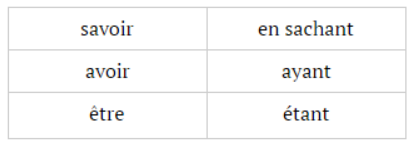
\includegraphics[scale=0.8]{charts/participePresentIrregulars.png}
\end{figure} \vspace{0.5\baselineskip} 


\section{Le pass\'e simple}

The \textit{pass\'e simple} tense expresses an action completed in the past| often a brief action. It is very rare in spoken French. \vspace{0.5\baselineskip} 

E.g. \texttt{suddenly the cyclist fell to the ground. $\rightarrow$ soudain, le cycliste chuta par terre.} \vspace{0.5\baselineskip} 

ER and IR verbs follow a rather regular pattern, whereas RE verbs can fall into one of three models. Some irregular verbs follow models that do not agree with their infinitive endings.  \vspace{0.5\baselineskip} 

The following charts cover the regular verbs: 

\begin{figure}[H]
	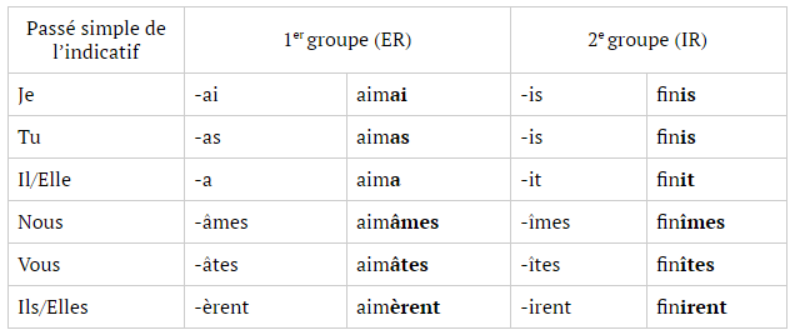
\includegraphics[scale=0.6]{charts/passeSimple1.png}
\end{figure} \vspace{0.5\baselineskip} 
\begin{figure}[H]
	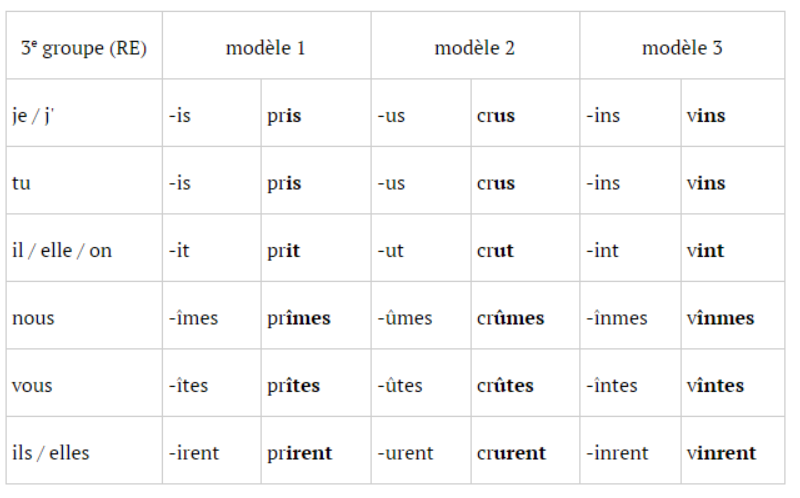
\includegraphics[scale=0.6]{charts/passeSimple2.png}
\end{figure} \vspace{0.5\baselineskip} 


\section{Le plus-que-parfait}

The \textit{plus-que-parfait} tense is used to indicate an action in the past that occurred before another action in the past. That which occurred later can either be explicit or implied. \vspace{0.5\baselineskip} 

For example, \texttt{he hadn't done his homework before playing video games. $\rightarrow$ il n'avait pas fait ses devoirs avant de jouer les jeux-vid\'eos.} \vspace{0.5\baselineskip} 

The \textit{plus-que-parfait} tense is conjugated by using an auxiliary of \textit{avoir} or \textit{\^etre} in the \textit{imparfait} tense (see section 1.6) and the \textit{participe pass\'e} of the verb to be used   (see section 1.3). \vspace{0.5\baselineskip} 

One construction of the \textit{plus-que-parfait} involves the pluperfect, (\textit{pass\'e compos\'e}) mentioned in section 1.4.  \vspace{0.5\baselineskip} 

For instance, \texttt{yesterday, I ate the sandwich that I had made the day before. $\rightarrow$ hier, j'ai mang\'e le sandwich que j'avais fait la veille.}  \vspace{0.5\baselineskip} 

\section{Le conditionnel pass\'e}

The \textit{conditionnel pass\'e} tense best corresponds to the use of “\textit{would have}” in English. In the sentence: ``\texttt{If I had won one million dollars, I would have bought a yacht.}”, the verb \textit{to buy} is said to be in the \textit{conditionnel pass\'e} tense. \vspace{0.5\baselineskip} 

The \textit{conditionnel pass\'e} is constructed using an auxiliary of \textit{avoir} or \textit{\^etre} in the \textit{conditionnel pr\'esent} tense (see section 1.8) and the \textit{participe pass\'e} (see section 1.3) of the main verb. \vspace{0.5\baselineskip} 

The \textit{si + imparfait \ldots conditionnel} construction mentioned in section 1.7 also applies to the \textit{conditionnel pass\'e} but with the \textit{plus-que-parfait} (section 1.11) in place of the \textit{imparfait}. \vspace{0.5\baselineskip} 

\section{Le futur ant\'erieur}

The \textit{futur ant\'erieur} is used to express a future action or event that will be completed before another future action or to describe a future action or event that will have been completed in the future. The tense best corresponds to the use of ``\textit{will have}” in English.\vspace{0.5\baselineskip} 

The \textit{futur ant\'erieur} is formed by the auxiliary of either \textit{avoir} or \textit{\^etre} in the \textit{futur simple} tense (see section 1.5) and the \textit{participe pass\'e} (see section 1.3). \vspace{0.5\baselineskip} 

One possible construction of the \textit{futur ant\'erieur} also involves the \textit{futur simple} (see section 1.5). The \textit{futur ant\'erieur} is used with a phrase such as \textit{apr\`es que} (after), \textit{aussit\^ot que} (as soon as), \textit{d\`es que} (as soon as), \textit{lorsque} (when), or \textit{quand} (when). The \textit{futur simple} component then expresses \textit{that which will have already happened by then}. \vspace{0.5\baselineskip}

For example, \texttt{when you arrive, he will already have done it. $\rightarrow$ quand tu arriveras, il l'aura d\'ej\`a fait.}

\section{Les verbes pronominaux}

Pronominal verbs consist of a personal (reflexive) pronoun in addition to the subject pronoun because the subject(s) performing the task are the same as the objects being are acted upon.  They can be used to express reflexive action, reciprocated action, and they are sometimes necessary for idiomatic pronominal verbs. \vspace{0.25\baselineskip}

In the present tense, pronominal verbs conjugate in the same way as non-pronominal verbs. The only difference is that pronominal verbs require the above mentioned reflexive pronoun. The reflexive pronoun depends on the subject pronoun. In the case of \textit{il}, (he), the desired reflexive pronoun is \textit{se}.  \vspace{0.5\baselineskip}

\newpage The subject pronouns and their respective reflexive pronouns are given as follows:

\begin{figure}[H]
	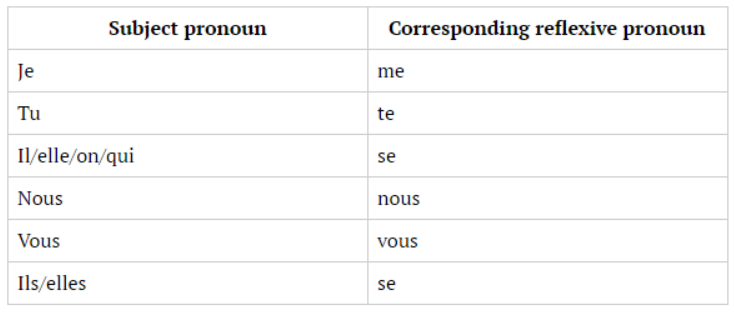
\includegraphics[scale=0.6]{charts/reflexivePronouns.png}
\end{figure} \vspace{0.5\baselineskip} 

Note that only certain verbs are conjugated in this way| pronominal verbs. For example, \textit{se marier, se lever, se laver} are all conjugated in the above manner, but not anything like \textit{aller,} or \textit{aider}. Notice that the infinitive form of a pronominal verb includes the \textit{se}. \vspace{0.5\baselineskip}

Reflexive pronominal verbs are the actions that a subject(s) does to him or herself. This includes washing oneself (\textit{se laver}), walking oneself (\textit{se promener}), introducing oneself (\textit{se pr\'esenter}), feeding oneself (\textit{se nourrir}), applying makeup to oneself (\textit{se maquiller}) and more.  \vspace{0.5\baselineskip}

Reciprocal pronominal verbs are the actions that subjects do to each other. For example, \texttt{we know each other well $\rightarrow$ nous nous connaissons bien}. \vspace{0.5\baselineskip}

Idiomatic pronominal verbs do not fit into the previous two categories, but are also conjugated with a reflexive pronoun. For example, \textit{se trouver}.  \vspace{0.5\baselineskip}

Negation with pronominal verbs involves \textit{ne} and its partner, usually \textit{pas} (similar to regular negation), but they also sandwich the reflexive pronoun. \vspace{0.5\baselineskip} 

For example, \texttt{je ne me l\`eve pas t\^ot; nous ne nous connaissons pas}. \vspace{0.5\baselineskip}

\section{Les verbes pronominaux au pass\'e compos\'e}

Pronominal verbs in the \textit{pass\'e compos\'e} (see section 1.4) are formed using \textit{\^etre} as an auxiliary. As with compound tenses and direct objects, the reflexive pronouns (\textit{me, te, se,} etc.) are placed immediately before the auxiliary. \vspace{0.5\baselineskip} 

For example, in the present tense ``\texttt{I wash myself}" translates to ``\texttt{je me lave}". In the pluperfect tense, ``\texttt{I washed myself}" translates to ``\texttt{je me suis lav\'e}".  Note that there must be an agreement between the gender and number of the subject, and the verb ending. \vspace{0.5\baselineskip}

For instance, \texttt{she washed herself $\rightarrow$ elle s'est lav\'ee}. \vspace{0.5\baselineskip} 

Negation occurs when \textit{ne} and its partner, usually \textit{pas}, sandwich the reflexive pronoun and the auxiliary. E.g., \texttt{Ils \textcolor{red}{ne} se sont \textcolor{red}{pas} ras\'es}. \vspace{0.5\baselineskip} 

\section{L'imp\'eratif}

The imperative mood expresses a command. In French, the \textit{imp\'eratif} is only conjugated for three subjects: second person singular (you, \textit{tu}), second person plural (second person singular, respectful) (you, \textit{vous}), and first person plural (we, \textit{nous}).  \vspace{0.5\baselineskip} 

The regular verbs in this tense are generally identical to their present tense counterparts. Note though, that the \textit{imp\'eratif} is not used with a subject pronoun. \vspace{0.5\baselineskip} 

For example, \texttt{finish! $\rightarrow$ finis!} \vspace{0.5\baselineskip} 

However, in the case of ER verbs in the second person singular (you, \textit{tu}) form, the final \textit{-s} is removed from the present tense form. \vspace{0.5\baselineskip} 

For instance, \texttt{talk! $\rightarrow$ parle!} \vspace{0.5\baselineskip} 

Other irregular verbs include:  \vspace{0.5\baselineskip} 

\begin{itemize}
	\item Savoir
	\item Avoir
	\item \^Etre 
	\item Vouloir
\end{itemize}

\chapter{Adjectives}
\section{Introduction}
An adjective modifies or describes a noun. For example, in the sentence \textit{I drive a blue car}, we can use the word \textit{blue} to figure out the colour of the car. Notice that the adjective, in this case, precedes the noun— in English, that is the norm. \vspace{0.5\baselineskip}

However, in French, the majority of adjectives come after the noun, with the exception of certain adjectives that describe certain characteristics. This includes beauty, age, goods, or size, or B.A.G.S., for short. Note though, that not all adjectives in these categories are placed before the noun. For example, gigantic in French, \textit{gigantesque}, is still placed after the noun. \vspace{0.5\baselineskip}

There is a French equivalent of the B.A.G.S. acronym: B.A.T.O.N., which stands for \textit{beaut\'e, \^age, taille (size), bont\'e (goodness), nombr\'e}. \vspace{0.5\baselineskip}

For example, \texttt{a bad storm $\rightarrow$ un mauvais orage}.
As opposed to \texttt{a blue car $\rightarrow$ une voiture bleue}. \vspace{0.5\baselineskip}

Note that there must be an agreement between gender and number of the noun, and the adjective. If the noun is feminine and plural, the adjective had better show that. E.g., \texttt{some little girls $\rightarrow$ des petites filles}— note the -s. \vspace{0.5\baselineskip}


Sometimes, the placement of the adjective even affects the meaning of the modification! For example, when \textit{dernier} is placed before a noun it means \textit{final}, but when it is placed after the noun it means \textit{previous} or \textit{last}.  \vspace{0.5\baselineskip}

\section{Formation}

Different adjectives follow different models that distinguish masculine and feminine forms. For example, the singular masculine form of the word lucky is \textit{chanceux}. Its corresponding singular feminine form is \textit{chanceuse}. \textit{Chanceux} follows the \textit{-x \ldots -se}  model. \vspace{0.5\baselineskip}

Consider these common models:  \vspace{0.5\baselineskip}

\begin{figure}[H]
	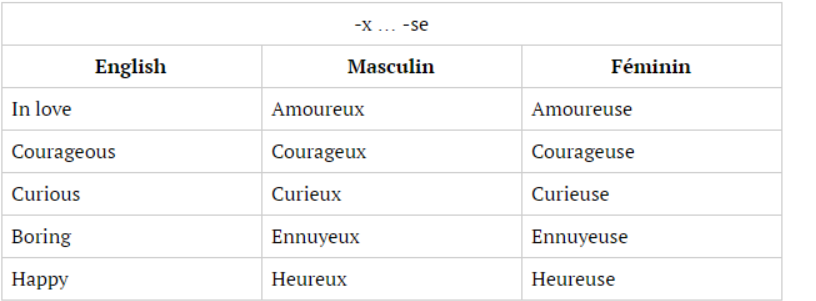
\includegraphics[scale=0.6]{charts/adjective1.png}
\end{figure} \vspace{0.5\baselineskip}

\begin{figure}[H]
	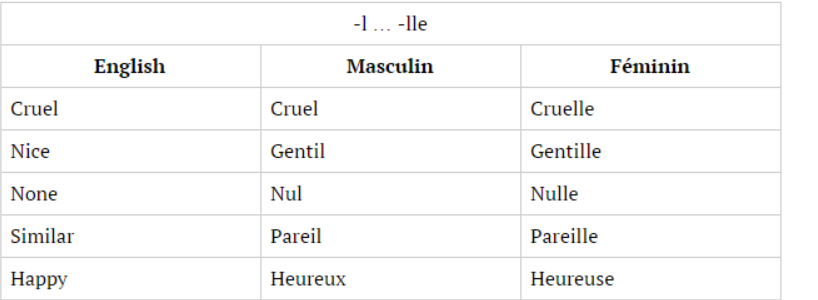
\includegraphics[scale=0.6]{charts/adjective2.png}
\end{figure} \vspace{0.5\baselineskip}

\begin{figure}[H]
	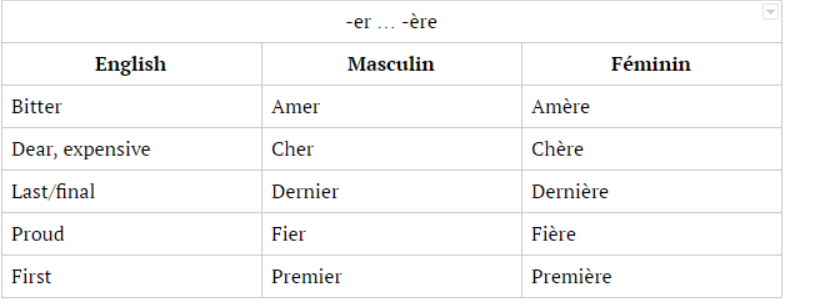
\includegraphics[scale=0.6]{charts/adjective3.png}
\end{figure} \vspace{0.5\baselineskip}

Here are some rather irregular adjectives and their various forms: 

\begin{figure}[H]
	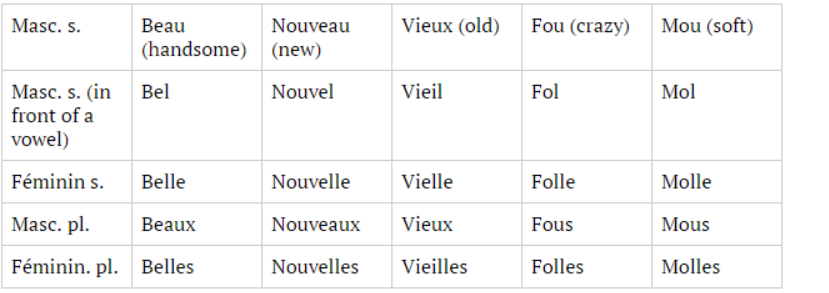
\includegraphics[scale=0.6]{charts/adjectiveIrregulars.png}
\end{figure} \vspace{0.5\baselineskip}

{\let\thefootnote\relax\footnote{Notice the second row (from the top) of the bottom-most chart. When the adjective ends in a vowel, there is generally an alternative form that ends in a consonant. This alternative form is used so that the construction is more pronounceable.}


\chapter{Pronouns}
\section{Object pronouns}

Object pronouns replace nouns in a sentence. The object pronouns can be divided into two categories, direct and indirect. 

\begin{figure}[H]
	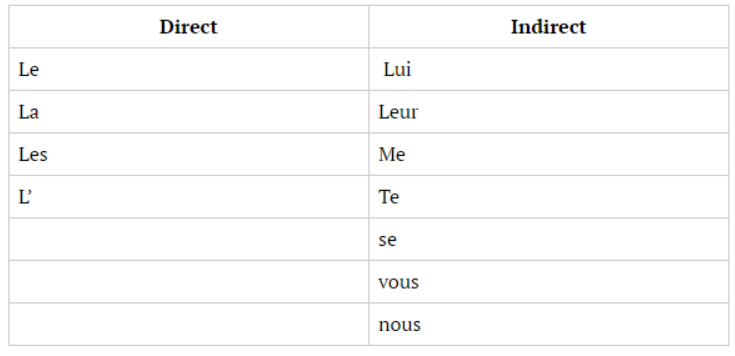
\includegraphics[scale=0.6]{charts/directAndIndirect.png}
\end{figure} \vspace{0.5\baselineskip} 

The difference between direct and indirect object pronouns is that direct object pronouns replace the direct object, the noun that receives the verb. Eg. \texttt{Il frappe le ball}. \textit{Le ball} in this sentence is the direct object. To replace the direct object in this  sentence we use \textit{le} since \textit{ball} is masculine: \textit{Il le frappe}. \textit{La} replaces feminine nouns and \textit{les} replaces plural nouns. If the noun begins with a vowel and is singular in number, a liaison is made with \textit{l'}. \vspace{0.5\baselineskip}

Indirect object pronouns are used in replacing indirect objects. In other words the noun which receives the direct object. E.g., \texttt{il donne le bal au gar\c{c}on}. In this sentence le gar\c{c}on is the indirect object pronoun. In french the indirect object is always followed by the preposition \textit{\`a}  in some form (\textit{au, à la, aux}). In order to replace \textit{au gar\c{c}on} in the sentence we use \textit{lui}: \texttt{il lui donne le ball}.  \vspace{0.5\baselineskip}

As shown in the above examples, object pronouns are placed immediately before the verb in the simple tenses. In compound tenses one places the object pronouns before the auxiliary.    \vspace{0.5\baselineskip}

\section{Agreement with object pronouns}

When forming complex tenses using the auxiliary verb \textit{avoir} we must only account for agreement when working with direct object pronouns.  \vspace{0.5\baselineskip}

For example, \texttt{ I had given these to the boy. $\rightarrow$ je les avais donn\'es au gar\c{c}on}.  \vspace{0.5\baselineskip}

If the pronoun is plural we must add \textit{-s} as appropriate(as seen in the example). If the pronoun is feminine we must add an \textit{-e} to the \textit{participe pass\'e} as appropriate: \textit{Je l'avais donn\'ee}. If the pronoun is masculine we don't add anything and if the pronoun is both feminine \textit{and} plural we must add \textit{-es}.  \vspace{0.5\baselineskip}
\newpage
\section{Ordering of object pronouns}

Consider the following diagram that shows the order (from left to right) of the use of object pronouns.

\begin{figure}[H]
	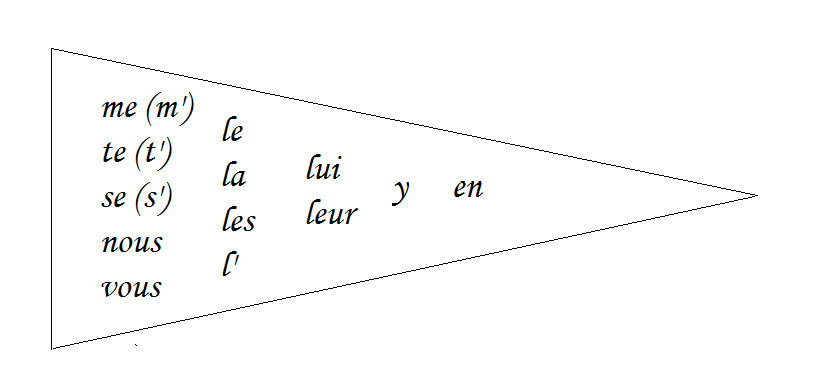
\includegraphics[scale=0.6]{charts/objectorder.png}
\end{figure} \vspace{0.5\baselineskip} 

For example, \texttt{\textcolor{orange}{I} \textcolor{red}{gave} \textcolor{cyan}{it} \textcolor{magenta}{to them} $\rightarrow$ \textcolor{orange}{je} \textcolor{cyan}{le} \textcolor{magenta}{leur} \textcolor{red}{ai donn\'e}}. \vspace{0.5\baselineskip}

Negation can be confusing. \textit{Ne} and its partner, usually \textit{pas}, sandwich all the object pronouns, and the auxiliary if applicable. Otherwise, \textit{ne} and its partner sandwich everything. Note that the placement of the object pronouns is also very important. In compound tenses (and constructions with two verbs), the object pronouns immediately proceed the second verb (in the infinitive form).\vspace{0.5\baselineskip}

For example, \texttt{\textcolor{orange}{I} \textcolor{green!50!orange}{am} \textcolor{red}{not} \textcolor{green!50!orange}{going to} \textcolor{magenta!70}{say} \textcolor{cyan}{it} \textcolor{blue}{to them} $\rightarrow$ \textcolor{orange}{je} \textcolor{red}{ne} \textcolor{green!50!orange}{vais} \textcolor{red}{pas} \textcolor{cyan}{le} \textcolor{blue}{leur} \textcolor{magenta!70}{dire}}. \vspace{0.5\baselineskip} 

In tenses with a single conjugated element, the object pronouns are simply placed before the verb, and if there is a negation, before the second part of the negation e.g., \textit{pas, assez, aucun, plus,} etc. \vspace{0.5\baselineskip}

\section{Relative pronouns}

Relative pronouns are used to describe nouns that may not have been explicitly mentioned. For example, if I started a conversation by saying ``\texttt{what really bothers me is [...]}", the word, \textit{what}, would refer to something that had not previously been mentioned at all. \vspace{0.5\baselineskip}

	Also, if I wanted to say ``\texttt{the computer that I use}", the word ``\textit{that}" is replaced with a relative pronoun. If I wanted to say ``\texttt{the guy who punched me}", the word, ``\textit{who}, which now joins a subject pronoun (the guy is performing the action: punching me) to the verb (instead of an object pronoun (the computer was being used by me) to a subject pronoun). \vspace{0.5\baselineskip}
	
In other words, when the relative pronoun deals with an object, it follows that object and is followed \textbf{by} a subject. In this case, \textit{computer} is followed by \textit{that} (the relative pronoun), which is followed by \textit{I} (the subject). \vspace{0.5\baselineskip}

When the relative pronoun deals with a subject, it follows the subject and is followed \textbf{by} the verb. In this case, \textit{guy} is followed by \textit{who} (the relative pronoun), which is followed by \textit{punched} (the verb). \vspace{0.5\baselineskip}

	In French, relative pronouns depend on the type of noun that they are dealing with: whether they are subjects, objects, or places. \vspace{0.5\baselineskip}

	\textit{Que} is used to join the object to the subject. It translates to \textit{that, whom, or which}. \vspace{0.5\baselineskip}

	For example, \texttt{the food that I bought tasted awful $\rightarrow$ la nourriture que j'ai achet\'e \'etait affreuse}.  \vspace{0.5\baselineskip}

	\textit{Qui} is used to join the subject to the verb. It translates to \textit{that, who, or which}. \vspace{0.5\baselineskip}

	For example, \texttt{the teacher who yelled at me $\rightarrow$ le professeur qui criait sur moi}. \vspace{0.5\baselineskip}

	\textit{O\`u} is used to join a place or time and a subject. It translates to \textit{where, or when}. \vspace{0.25\baselineskip}

	For example, \texttt{the playground where I hurt myself $\rightarrow$ le terrain de jeu o\`u je me suis bless\'e}. \vspace{0.5\baselineskip}

	\textit{Dont} is tricky. Since the French abide by the “don't end your sentences with a preposition” rule (from Latin), \textit{dont} is used when there are expressions ending in \textit{de}, which is a preposition. For example, \texttt{parler de} means to talk about. \vspace{0.5\baselineskip}

	``\texttt{The movie that I talked about}” would, according to our previously established relative pronouns, translate to ``\texttt{le film que j'ai parl\'e de}. However, because of the preposition rule, this construction would be unacceptable. The correct translation uses \textit{dont}: \texttt{le film dont j'ai parl\'e}.  \vspace{0.5\baselineskip}

	Some other expressions ending in de include: \textit{avoir peur de, s'agir de, \^etre fier de,} and \textit{promettre de}. \vspace{0.5\baselineskip}


\section{Demonstrative pronouns}

Demonstrative pronouns are used to ``point” or refer to nouns. In English, the demonstrative pronouns are \textit{this one, that one, these,} and \textit{those}. For each gender and number combination, there is a demonstrative pronoun: \vspace{0.5\baselineskip}


\begin{figure}[H]
	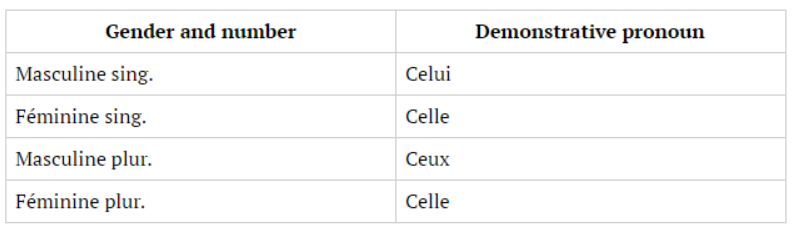
\includegraphics[scale=0.6]{charts/demonstrativePronouns.png}
\end{figure} \vspace{0.5\baselineskip} 

Demonstrative pronouns cannot stand alone. They must be used with one of the following constructions:

\begin{description}
	\item[1.  With a suffix.] If we want to say``\texttt{this one here}, or ``\textit{that one there}, we could say \texttt{celui-ci} and \texttt{celui-l\`a}, respectively, where \textit{ci} means \textit{here}, and the \textit{l\`a} means \textit{there}.
		
		For example, \texttt{which girl did it, this one, or that one? $\rightarrow$ Quelle fille l'a fait, celle-ci ou celle-l\`a?}
		
	\item[2. In a prepositional phrase.] If we want to say ``\texttt{that of [...]}" or ``\texttt{those of [...]}", we also use demonstrative pronouns by simply attaching a \textit{de} to the end. 

		For example, \texttt{which team are you cheering for, that of France, or that of England? $\rightarrow$ Quelle \'equipe est-ce que tu soutiens, celle de la France, ou celle de l'Angleterre?}
		
	\item[3. With a relative pronoun (see section 3.3).] In English, the equivalent in this scenario is ``\texttt{he who [...]}"  or ``\texttt{whoever [...]}". 
	
		For example, \texttt{he who lied will be punished. $\rightarrow$ celui qui a menti sera puni.}

\end{description}

In addition to these four gender and number based demonstrative pronouns, French also offers a few indefinite demonstrative pronouns, which are impersonal and do not have different forms for different genders and numbers. These indefinite demonstrative pronouns are: \vspace{0.5\baselineskip}


\begin{description}
	\item[1. Ce] | \textit{this or that}. Usually use with \textit{\^etre}.
	
	For example, \texttt{that's a good idea! $\rightarrow$ c'est une bonne id\'ee!}
	
	\item[2. Cela] | a contraction of \textit{ce} and \textit{l\`a} (\textit{this} and \textit{there}). 
	
	For example, \texttt{that makes me happy $\rightarrow$ cela me fait plaisir!}
	
	\item[3. Ceci] | a contraction of \textit{ce} and \textit{ici} (\textit{this} and \textit{here}). 
	
	For example, \texttt{this is going to be easy $\rightarrow$ ceci va \^etre facile.}
	
	\item[4. \c{C}a] |  the informal replacement of both \textit{ceci} and \textit{cela} (both of which are relatively rare).
	
	For example, \texttt{that makes me happy $\rightarrow$ \c{c}a me fait plaisir!}
\end{description}
		
\appendix 
\chapter{Expressions}

\noindent \^etre aux oiseaux $\rightarrow$ To be very happy \\
se mettre dans la peau d'un astronaute $\rightarrow$ To be on top of the world \\
\^etre dans les nuages $\rightarrow$ To be in the clouds \\
\^etre au m\^eme longueur d'onde $\rightarrow$ To be on the same wavelength \\
\^etre sur les dents $\rightarrow$ To be on edge \\
\^etre au mercredi des cendres. $\rightarrow$ To be depressed \\
avoir h\^ate de $\rightarrow$ To be eager to \\
ne pas en revenir$\rightarrow$ To be not able to get over it \\
ce n'est pas la mer \'a boire $\rightarrow$ I'm not asking you to drink the ocean/ it's not the most difficult thing in the world! \\
qu'elle mouche l'avait piqu\'e $\rightarrow$ What has gotten into him \\
il y a une lumi\`ere au but du tunnel $\rightarrow$ There is a light at the end of the tunnel \\
sain et sauf $\rightarrow$ safe and sound \\
avoir pour but de $\rightarrow$ to aim to do \\

\chapter{Vocabulary}

Quizlets for reading selections found in the Nouvelles fronti\`res Anthologie ($11^{e}$):

	\indent \indent https://goo.gl/U2RQpu
\end{document}